\documentclass[conference]{IEEEtran}

\usepackage{newtxtext,newtxmath}
\usepackage{amsmath}
\usepackage{booktabs}
\usepackage{graphicx}
\usepackage{xcolor}
\usepackage{url}
\usepackage[hidelinks]{hyperref}
\hypersetup{
  pdftitle={QuaRM: Supplementary Material and Artifact Guide},
  pdfauthor={AUTHOR METADATA REQUIRED BEFORE SUBMISSION},
  pdfsubject={Supplement to an ICDE 2027 regular research submission},
  pdfkeywords={data quality, artifact, reproducibility, Shapley value}
}

\graphicspath{{../../artifacts/icde_figures/}{../../artifacts/figures/}}
% Generated by scripts/make_icde_paper_assets.py; do not edit manually.
\newcommand{\NYCRisk}{19.20}
\newcommand{\NYCDimensionDebt}{9.56}
\newcommand{\NYCDimensionLow}{8.45}
\newcommand{\NYCDimensionHigh}{10.73}
\newcommand{\MaxRelInteraction}{5.90}
\newcommand{\MLPositive}{7}
\newcommand{\MLSettings}{8}
\newcommand{\MLMaxInteraction}{2.03}
\newcommand{\SamplingTopSixtyFour}{95.8}
\newcommand{\SamplingSurfaceSixtyFour}{12.8}
\newcommand{\SamplingRMSESixtyFour}{0.206}
\newcommand{\SamplingTopOneTwentyEight}{99.0}
\newcommand{\SamplingSurfaceOneTwentyEight}{22.4}
\newcommand{\SamplingRMSEOneTwentyEight}{0.142}

\newcommand{\TODO}[1]{\textcolor{red}{\textbf{[#1]}}}

\title{QuaRM: Accounting for Data-Quality Debt Across\\
Interacting Defects and Analytical Workloads\\
{\large Supplementary Material and Artifact Guide}}

\author{\IEEEauthorblockN{\TODO{AUTHOR NAMES REQUIRED---SINGLE-BLIND SUBMISSION}}
\IEEEauthorblockA{\TODO{Affiliations, emails, and ORCIDs required before submission}}}

\begin{document}
\maketitle

This supplement expands the experimental record for the ICDE 2027 submission. It is not an appendix to the 12-page paper and contains no claim required to understand the main argument. Every table is generated directly from the checked-in result CSVs by \texttt{scripts/make\_icde\_paper\_assets.py}.

\section{Artifact map}

The public release must expose the following structure:

\begin{itemize}
  \item \texttt{src/quarm}: exact attribution, sampling, ML, and relational backends;
  \item \texttt{experiments}: frozen study drivers and paired-design ablation;
  \item \texttt{artifacts/icde\_results}: raw coalition observations, allocations, interactions, query allocations, scale, sampling, and SHA-256 manifests;
  \item \texttt{artifacts/results}: ML confirmation evidence and manifest;
  \item \texttt{paper/icde2027}: IEEEtran sources and generated evidence tables;
  \item \texttt{tests}: deterministic unit and integration tests; and
  \item \texttt{scripts}: official-data fetcher, asset generator, PDF QA, and submission audit.
\end{itemize}

Raw NYC inputs are not duplicated in the repository. \texttt{scripts/fetch\_public\_data.py} downloads them from the official TLC endpoint and rejects files whose hashes differ from the frozen January 2025 snapshot.

\section{Mechanisms and query workload}

\begin{table*}[t]
\caption{Relational experimental contract. All selected units are deterministic functions of the master seed, repeat, and mechanism name.}
\label{tab:contract}
\centering\small\setlength{\tabcolsep}{6pt}
\begin{tabular}{lll}
\toprule
Mechanism & unit selected at severity $\theta$ & transformation \\
\midrule
missing measures & monetary fact cells & replace with SQL NULL \\
value noise & monetary fact cells & multiply by a stochastic scale perturbation \\
orphan foreign keys & fact foreign-key cells & replace with an absent identifier \\
stale timestamps & fact event times & shift backward according to the fixed operator \\
dimension drift & selected dimension members & replace the analytical category/region label \\
duplicate facts & fact rows & append exact row copies after value-level mechanisms \\
\bottomrule
\end{tabular}
\end{table*}

The eight workload templates are: average order value by customer segment; customer count by region; daily revenue; order count by status; refund rate by region; revenue by product category; monthly revenue; and revenue by region. Each answer is aligned on group keys with absent groups filled by zero. The loss is clipped normalized $L_1$ error, and workload loss is the unweighted mean. Query-level allocations are retained in \texttt{query\_attributions.csv} and \texttt{nyc\_query\_attributions.csv}.

\section{Complete relational results}

% Generated by scripts/make_icde_paper_assets.py; do not edit manually.
\begin{table*}[t]
\caption{Complete relational Shapley allocations. Values and intervals are workload risk points; rank is the paired-bootstrap probability of being the largest account.}
\label{tab:supp-rel}
\centering\small\setlength{\tabcolsep}{6pt}
\begin{tabular}{llrrrr}
\toprule
Reference & mechanism & debt & 95\% low & 95\% high & rank-one (\%) \\
\midrule
NYC Taxi & dimension drift & 9.56 & 8.45 & 10.73 & 100.0 \\
NYC Taxi & stale time & 3.32 & 3.30 & 3.35 & 0.0 \\
NYC Taxi & duplicate facts & 2.55 & 2.00 & 3.12 & 0.0 \\
NYC Taxi & orphan keys & 1.63 & 0.95 & 2.51 & 0.0 \\
NYC Taxi & value noise & 1.22 & 1.00 & 1.59 & 0.0 \\
NYC Taxi & missing measures & 0.91 & 0.86 & 0.96 & 0.0 \\
\addlinespace
Uniform & duplicate facts & 2.27 & 2.22 & 2.33 & 100.0 \\
Uniform & value noise & 1.94 & 1.83 & 2.05 & 0.0 \\
Uniform & stale time & 1.87 & 1.84 & 1.90 & 0.0 \\
Uniform & orphan keys & 0.43 & 0.40 & 0.46 & 0.0 \\
Uniform & dimension drift & 0.41 & 0.33 & 0.51 & 0.0 \\
Uniform & missing measures & 0.27 & 0.21 & 0.32 & 0.0 \\
\addlinespace
Skewed & duplicate facts & 2.39 & 2.32 & 2.46 & 94.7 \\
Skewed & value noise & 1.98 & 1.89 & 2.06 & 0.0 \\
Skewed & stale time & 1.89 & 1.87 & 1.92 & 0.0 \\
Skewed & dimension drift & 1.77 & 1.06 & 2.56 & 5.3 \\
Skewed & orphan keys & 0.57 & 0.51 & 0.63 & 0.0 \\
Skewed & missing measures & 0.24 & 0.18 & 0.30 & 0.0 \\
\addlinespace
Seasonal & duplicate facts & 2.26 & 2.20 & 2.32 & 100.0 \\
Seasonal & stale time & 1.91 & 1.87 & 1.94 & 0.0 \\
Seasonal & value noise & 1.90 & 1.82 & 1.97 & 0.0 \\
Seasonal & dimension drift & 0.44 & 0.39 & 0.50 & 0.0 \\
Seasonal & orphan keys & 0.44 & 0.42 & 0.46 & 0.0 \\
Seasonal & missing measures & 0.28 & 0.23 & 0.34 & 0.0 \\
\addlinespace
\bottomrule
\end{tabular}
\end{table*}
\begin{table*}[t]
\caption{Complete ML confirmation study at 15\% prevalence. Debt and maximum interaction are bounded clean-test risk points.}
\label{tab:supp-ml}
\centering\small\setlength{\tabcolsep}{5pt}
\begin{tabular}{llrrlrrl}
\toprule
Dataset & model & rows & debt & top account & top prob. (\%) & $\max|I|$ & full-context best \\
\midrule
breast cancer & logistic & 569 & 3.80 & target noise & 98.2 & 1.42 & target noise \\
breast cancer & forest & 569 & 1.12 & missing cells & 68.3 & 0.39 & missing cells \\
wine & logistic & 178 & 6.48 & target noise & 99.8 & 2.03 & target noise \\
wine & forest & 178 & 1.70 & target noise & 78.2 & 0.54 & target noise \\
diabetes & ridge & 442 & 4.21 & feature noise & 100.0 & 0.96 & feature noise \\
diabetes & forest & 442 & 1.42 & feature noise & 59.2 & 0.31 & feature noise \\
synthetic nonlinear & logistic & 900 & -1.33 & missing cells & 54.8 & 0.58 & target noise \\
synthetic nonlinear & forest & 900 & 7.28 & feature noise & 99.1 & 1.65 & feature noise \\
\bottomrule
\end{tabular}
\end{table*}


Exact Shapley efficiency residual is zero for every relational population. The normalized Banzhaf residuals are $-1.89$ risk points for NYC and between $-1.40$ and $-1.56$ for the generated references. The largest absolute pairwise interactions are 5.62 (NYC), 5.87 (Uniform), 5.69 (Skewed), and 5.90 (Seasonal) points. In all four, missing measures and duplicate facts form the largest-magnitude pair.

\begin{figure*}[t]
\centering
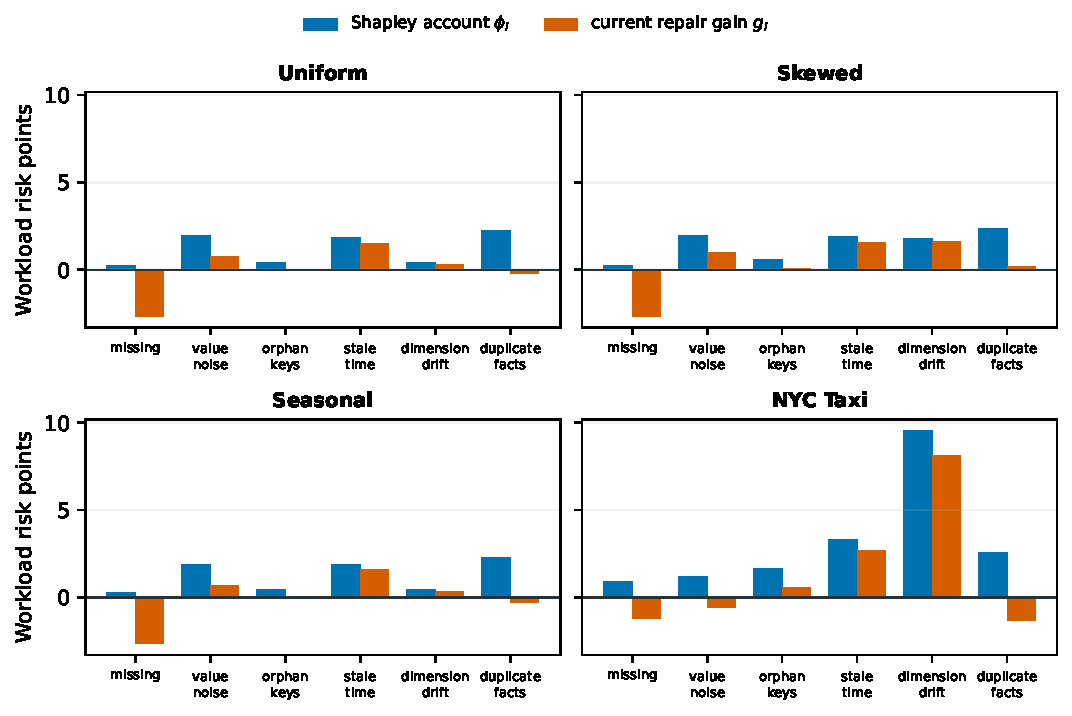
\includegraphics[width=0.94\textwidth]{icde_figure4_accounting_decision.pdf}
\caption{The complete accounting/intervention comparison. The underlying coalition means and every full-context marginal are available in the raw observations.}
\end{figure*}

\section{Scale and estimator details}

% Generated by scripts/make_icde_paper_assets.py; do not edit manually.
\begin{table}[t]
\caption{Controlled 12-mechanism permutation study (400 trials per budget).}
\label{tab:supp-sampling}
\centering\small\setlength{\tabcolsep}{6pt}
\begin{tabular}{rrrr}
\toprule
$B$ & median RMSE & top-one (\%) & surface (\%) \\
\midrule
4 & 0.823 & 48.5 & 1.1 \\
8 & 0.583 & 59.2 & 2.1 \\
16 & 0.411 & 72.5 & 3.9 \\
32 & 0.294 & 84.0 & 7.1 \\
64 & 0.206 & 95.8 & 12.8 \\
128 & 0.142 & 99.0 & 22.4 \\
256 & 0.100 & 100.0 & 37.1 \\
512 & 0.072 & 100.0 & 57.2 \\
\bottomrule
\end{tabular}
\end{table}


The exact row-scale experiment performs 64 coalition materializations and 512 SQL query executions per size. Wall times are 9.55~s at 10K facts, 22.17~s at 100K, and 97.22~s at 1M. These values include Python intervention, DuckDB ingestion, query evaluation, and answer comparison. They were collected on the environment recorded in \texttt{artifacts/icde\_results/manifest.json}.

For permutation sampling, each random order visits $m+1$ prefixes. A process-local cache ensures a coalition is evaluated at most once. The result object records sample count, marginal matrix, standard errors, exact coalition count, unique coalition count, and the simultaneous Hoeffding radius. The controlled surface contains unequal main effects, eight pair interactions, and three triple interactions followed by a logistic map; all 4,096 losses are therefore in $(0,1)$ and available for exact ground truth.

\begin{figure}[t]
\centering
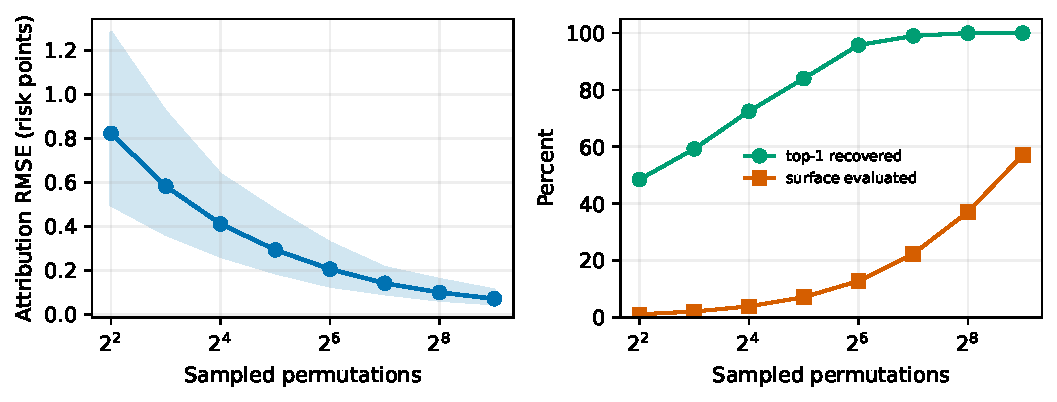
\includegraphics[width=\columnwidth]{icde_figure4_sampling_m12.pdf}
\caption{Estimator convergence and actual coalition coverage for the 12-mechanism study.}
\end{figure}

\section{ML confirmation}

The ML study follows the same paired-coalition contract with four mechanisms: missing cells, numeric feature noise, target noise, and duplicate rows. Every setting evaluates all 16 coalitions for 12 paired train/test splits. Seven of eight aggregate debts are positive; the nonlinear-synthetic/logistic setting is negative because feature noise acts as regularization for the fixed misspecified learner. This signed case is retained rather than clipped.

\section{Reproduction protocol}

On Windows PowerShell, after creating the environment and installing the project:

{\scriptsize
\begin{verbatim}
.venv\Scripts\python.exe -m pytest
.venv\Scripts\python.exe scripts\fetch_public_data.py
.venv\Scripts\python.exe experiments\run_study.py
.venv\Scripts\python.exe experiments\run_icde_study.py
.venv\Scripts\python.exe experiments\run_icde_real.py
.venv\Scripts\python.exe experiments\run_sampling_scalability.py
.venv\Scripts\python.exe experiments\analyze_paired_design.py
.venv\Scripts\python.exe scripts\make_icde_paper_assets.py
\end{verbatim}
}

The expensive full relational study requires approximately 15 minutes on the recorded laptop-class environment; the exact NYC study requires approximately four minutes. The public release should preserve the evidence CSVs so reviewers can regenerate all manuscript tables and figures without rerunning expensive workloads, then selectively reproduce any study.

\section{Artifact claims and checks}

The artifact supports the following independently checkable claims:

\begin{enumerate}
  \item all exact games contain every coalition exactly once per repeat;
  \item Shapley allocations close aggregate debt to floating-point precision;
  \item identical master seeds replay identical corruption selections and losses;
  \item a mechanism's random realization is invariant to coalition membership;
  \item the NYC inputs match pinned hashes from the official source;
  \item every paper number is generated from machine-readable evidence;
  \item every final PDF page is rendered and checked for page-bound violations; and
  \item the wheel, source distribution, tests, and paper sources are included in the release manifest.
\end{enumerate}

The release should be assigned a DOI or immutable repository tag before submission. A mutable branch URL is insufficient for archival review.

\section*{Acknowledgment of AI-Generated Content}
OpenAI Codex was used to generate and revise portions of the Python implementation, experimental orchestration, figures, supplementary material, and manuscript text. Before submission, the listed authors must independently inspect the source, reproduce the evidence, verify the claims, and accept responsibility for the complete work. No AI system is an author.

\end{document}
